\documentclass{article}
\usepackage{cmap}
\usepackage[utf8]{inputenc}
\usepackage[english,ukrainian]{babel}
\usepackage{graphicx}
\usepackage{geometry}
\usepackage{listings}
\usepackage{indentfirst}
\usepackage{subfigure}
\usepackage{caption}
\usepackage{amsmath}
\geometry{
	a4paper,
	left=20mm,
	right=20mm,
	top=20mm,
	bottom=20mm
}
\lstset{
	extendedchars=\true,
	tabsize=4,
	language=python,
	showstringspaces=false,
	showtabs=false,
	frame=lrtb,
	columns=fixed,
	keepspaces,
	breaklines=true
}
\graphicspath{ {pictures} }
\setlength{\parindent}{4em}
\newcommand\subject{Чисельні методи}
\newcommand\lecturer{доцент кафедри ПЗ\\Мельник Н.Б.}
\newcommand\teacher{асистент кафедри ПЗ\\Гарматій Г.Ю.}
\newcommand\mygroup{ПЗ-16}
\newcommand\lab{9}
\newcommand\theme{Наближення функцій методом найменших квадратів}
\newcommand\purpose{Ознайомлення на практиці з методом найменших квадратів
	апроксимації (наближення) функцій}

\begin{document}
	\begin{large}
		\begin{titlepage}
			\thispagestyle{empty}
			\begin{center}
				\textbf{МІНІСТЕРСТВО ОСВІТИ І НАУКИ УКРАЇНИ\\
					НАЦІОНАЛЬНИЙ УНІВЕРСИТЕТ "ЛЬВІВСЬКА ПОЛІТЕХНІКА"}
			\end{center}
			\begin{flushright}
				Інститут \textbf{КНІТ}\\
				Кафедра \textbf{ПЗ}
			\end{flushright}
			\vspace{200pt}
			\begin{center}
				\textbf{ЗВІТ}\\
				\vspace{10pt}
				До лабораторної роботи № \lab\\
				\textbf{На тему}: “\textit{\theme}”\\
				\textbf{З дисципліни}: “\subject”
			\end{center}
			\vspace{90pt}
			\begin{flushright}
				
				\textbf{Лектор}:\\
				\lecturer\\
				\vspace{28pt}
				\textbf{Виконав}:\\
				
				студент групи \mygroup\\
				Коваленко Д.М.\\
				\vspace{28pt}
				\textbf{Прийняв}:\\
				
				\teacher\\
				
				\vspace{28pt}
				«\rule{1cm}{0.15mm}» \rule{1.5cm}{0.15mm} 2022 р.\\
				$\sum$ = \rule{1cm}{0.15mm}……………\\
				
			\end{flushright}
			\vspace{\fill}
			\begin{center}
				\textbf{Львів — 2022}
			\end{center}
		\end{titlepage}
		
		\begin{description}
			\item[Тема.] \theme.
			\item[Мета.] \purpose.
		\end{description}
		
		\section*{Теоретичні відомості}
		\subsection*{Інтерполяційний поліном Лагранжа}
		Наближену функцію $y=f(x)$ представимо у вигляді 
		\begin{gather}
			\varphi(x)=L_n(x)=\sum_{i=0}^{n}P_i(x)f(x_i),\nonumber
		\end{gather}
		де $P_i(x)$ такий многочлен, що
		
		\begin{gather}
			P_i(x_j)=\left\{\begin{array}{@{}l@{}}
				0, i \ne j\\\nonumber
				1, i = j\nonumber
			\end{array}\right.\,
			, \hspace{28pt} i, j=0,1...n.
		\end{gather}
	
		Оскільки точки $x_0, x_1, x_{i-1}, x_{i+1}, ..., x_n$ є коренями многочлена $P_i(x)$, то його можна записати наступним чином
		\begin{gather}
			P_i(x)=\frac{(x-x_0)(x-x_1)...(x-x_{i-1})(x-x_{i+1})...(x-x_n)}{(x_i-x_0)(x_i-x_1)...(x_i-x_{i-1})(x_i-x_{i+1})...(x_i-x_n)}\nonumber
		\end{gather}
		а наближена функція, яку називають інтерполяційним многочленом Лагранжа, матиме вигляд
		
		\begin{gather}
			\varphi(x)=L_n(x)=\sum_{i=0}^{n}\frac{(x-x_0)(x-x_1)...(x-x_{i-1})(x-x_{i+1})...(x-x_n)}{(x_i-x_0)(x_i-x_1)...(x_i-x_{i-1})(x_i-x_{i+1})...(x_i-x_n)}f(x_i)\nonumber
		\end{gather}
		
		Поліном Лагранжа для випадку рівновіддалених вузлів має вигляд
		\begin{gather}
			L_n(x)=\frac{1}{n!}\Pi_{n+1}(t)\sum_{i=0}^{n}(-1)^{n-i}\frac{C_n^i}{t-i}y_i\nonumber
		\end{gather}
		де
		\begin{gather}
			C_n^i=\frac{n!}{i!(n-i)!}\nonumber
		\end{gather}
		 
		\subsection*{Інтерполяційний поліном Ньютона}
		Для загального випадку нерівновіддалених вузлів поліном $P_i(x)$ записують у вигляді
		\begin{gather}\nonumber
			P_n(x)=f(x_0)+f(x_0, x_1)(x-x_0)+f(x_0,x_1,x_2)(x-x_0)(x-x_1)+\\
			+...+f(x_0,x_1,...,x_n)(x-x_0)(x-x_1)...(x-x_{n-1}),\nonumber
		\end{gather}
		де скінченна різниця n-го порядку
		\begin{gather}
			\Delta^nf(x_i)=\sum_{j=0}^{n}(-1)^jC_n^jf(i+j)\nonumber
		\end{gather}
		\section*{Лабораторне завдання}
		Використовуючи інтерполяційні поліноми Лагранжа та Ньютона,
		обчислити значення табличної заданої функції у точці $x_0 = 0.455$.
		\vspace{5pt}
		
		\begin{tabular}{|c|c|c|c|c|c|c|c|c|c|c|}
			\hline
			x & 0.45 & 0.46 & 0.47 & 0.48 & 0.49 & 0.50 & 0.51 & 0.52 & 0.53 & 0.54 \\
			\hline
			y & 20.19 & 19.61 & 18.94 & 18.17 & 17.30 & 16.31 & 15.19 & 13.94 & 12.55 & 10.99\\
			\hline
		\end{tabular}
	
		\section*{Хід роботи}
		У даної функції усі вузли $x$ рівновіддалені з кроком $0.01$.
		
		\begin{tabular}{|c|c|c|c|c|c|}
			\hline
			$x_i$ & $f(x_i)$ & $\varDelta f(x_i)$ & $\varDelta^2 f(x_i)$ & $\varDelta^3 f(x_i)$ & $\varDelta^4 f(x_i)$ \\
			$x_0$ & 20.19 & -0.58 & -0.09 & 0.19 & -0.19\\
			$x_1$ & 19.61 & -0.67 & 0.1  & 0 & -\\
			$x_2$ & 18.94 & -0.77 & 0.1 & - & -\\
			$x_3$ & 18.17 & -0.87 & - & - & -\\
			$x_4$ & 17.30 & - & - & - & -\\
			\hline
		\end{tabular}
		
		\subsection*{Інтерполяційний поліном Лагранжа}
		Використаю формулу
		
		\begin{gather}
			L_n(x)=\frac{1}{n!}\Pi_{n+1}(t)\sum_{i=0}^{n}(-1)^{n-i}\frac{C_n^i}{t-i}y_i\nonumber
		\end{gather}
	
		для знаходження полінома та підставлю $x_0=0.455$ в знайдений поліном щоб знайти значення фукції в цій точці.
			
		\noindent\textit{\textbf{Код програми} (файл lab\_\lab1.py):}
		\begin{lstlisting}
import numpy as np

def data_to_matrix(path):
	return (
		np.loadtxt(open(path, "rb"), delimiter=",")[0],
		np.loadtxt(open(path, "rb"), delimiter=",")[1],
	)

def lagrange(x, y, x0):
	n = np.shape(x)[0]
	yp = 0
	for i in range(n):
		p = 1
		for j in range(n):
			if i != j:
			p *= (x0 - x[j])/(x[i] - x[j])
			yp += p * y[i]    
	return yp

path = input("Введіть шлях до файлу з даними: ") or "data.csv"
x, y = data_to_matrix(path)
print(f"Результат полінома Лагранжа у точці x0=0.455: {round(lagrange(x, y, 0.455), 4)}.")\end{lstlisting}
		
		\subsection*{Інтерполяційний поліном Ньютона}
		
		Для знаходження полінома та підставлю $x_0=0.455$ в знайдений поліном щоб знайти значення фукції в цій точці.
		
		\noindent\textit{\textbf{Код програми} (файл lab\_\lab2.py):}
		\begin{lstlisting}
import numpy as np

def data_to_matrix(path):
	return (
		np.loadtxt(open(path, "rb"), delimiter=",")[0],
		np.loadtxt(open(path, "rb"), delimiter=",")[1],
	)

def newton(x, y, r):
	n = len(x)
	a = [y[i] for i in range(n)]
	for j in range(1, n):
		for i in range(n-1, j-1, -1):
			a[i] = (a[i] - a[i-1]) / (x[i] - x[i-j])
	
	n = len(a) - 1
	temp = a[n] + (r - x[n])
	for i in range(n - 1, -1, -1):
		temp = temp * (r - x[i]) + a[i]
	return temp

path = input("Введіть шлях до файлу з даними: ") or "data.csv"
x, y = data_to_matrix(path)
print(f"Результат полінома Ньютона у точці x0=0.455: {round(newton(x, y, 0.455), 4)}.")\end{lstlisting}
		
		\noindent\textit{\textbf{Файл даних} (data.csv):}
		\begin{lstlisting}
0.45, 0.46, 0.47, 0.48, 0.49, 0.50, 0.51, 0.52, 0.53, 0.54
20.19, 19.61, 18.94, 18.17, 17.30, 16.31, 15.19, 13.94, 12.55, 10.99\end{lstlisting}
		
		\begin{figure}[h!]
			\centering
			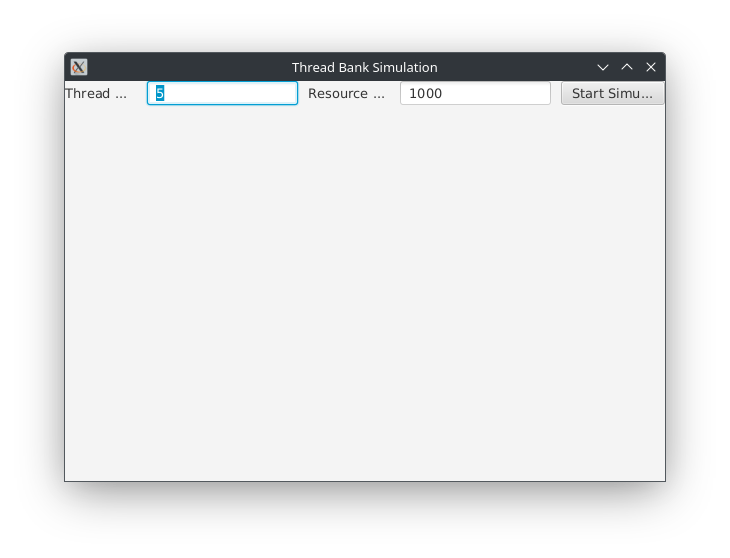
\includegraphics[scale=0.7]{1}
			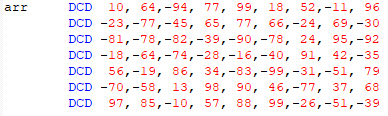
\includegraphics[scale=0.7]{2}
			\caption{Робота програми}
		\end{figure}
		
		\section*{Висновок}
		На лабораторній роботі я засвоїв практичні навички використання полінома Лагранжа та Ньютона для обчислення таблично заданої функції
		
		\begin{tabular}{|c|c|c|c|c|c|c|c|c|c|c|}
			\hline
			x & 0.45 & 0.46 & 0.47 & 0.48 & 0.49 & 0.50 & 0.51 & 0.52 & 0.53 & 0.54 \\
			\hline
			y & 20.19 & 19.61 & 18.94 & 18.17 & 17.30 & 16.31 & 15.19 & 13.94 & 12.55 & 10.99\\
			\hline
		\end{tabular}
		\vspace{5pt}\\
		у заданій точці $x_0=0.455$ та отримав результат 19.9046

	\end{large}
\end{document}
